%!TEX root = main.tex
% UTF-8 encoding

\section{Proposed Approach}
\label{sec:model}
We next discuss in detail our proposed euphemism detection approach in Section \ref{sec:model_det} and the proposed euphemism identification approach in Section \ref{sec:model_iden}. 


\subsection{Euphemism Detection}
\label{sec:model_det}
\begin{figure*}
	\centering
	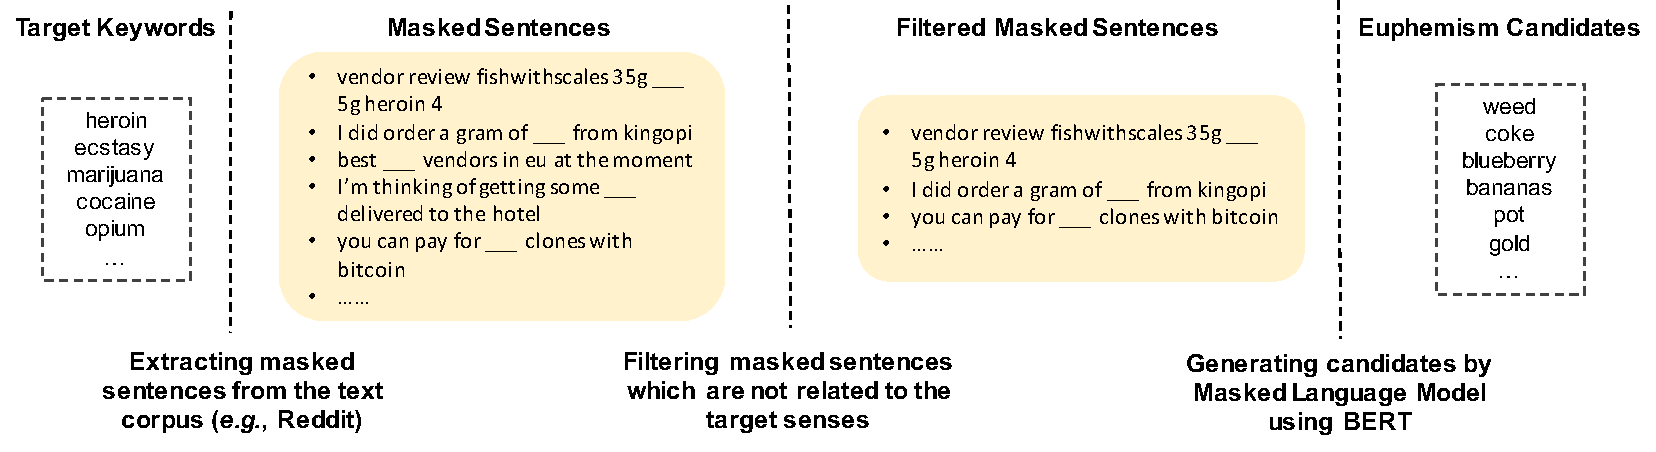
\includegraphics[width=1.0\linewidth]{figures/2}
	\caption{An overview of the euphemism detection framework.}
	\label{fig:model_det}
\end{figure*}

% The challenge to euphemism detection is that euphemisms are typically innocent-looking, and their usage in a sentence is often natural and grammatical. %lies in the inability to identify them without having an explicit mapping between the words and their implied meanings. 
% For instance, the words used as euphemisms with drug meanings tend to be words used in common parlance. 
%For example, ``blueberry'' could either mean a fruit, or marijuana depending on the context. Without the context, deciding whether a word is a euphemism or not would be impossible even for human experts. %For instance, \eg, 'one ounce of \textit{cheese}'). 
%\nicolasc{we said this already in the introduction, almost verbatim, do we need to repeat it here? by the same token, the proposed model (section III)  is useful but do we need to re-define euphemism detection and identification since we defined them in the introduction already?}
% Answer to Nicolas: changed it to a shorter version. 

% Human experts (or even non-experts to a large extent) typically rely on context to disambiguate the meaning of polysemous words. With this in mind,
% much contemporary work on  euphemism detection has mainly relied on the implicit contextual information available in static word embeddings (\eg, word2vec) in combination with network analysis (\eg, community detection) \cite{taylor2017surfacing,magu2018determining}, using sentiment lexicons \cite{felt2020recognizing}, and relying on semantic comparison across corpora \cite{yuan2018reading}. 
% However, the use of static word embeddings, which provides a single representation for a given word (without accounting for its polysemy), leads to an ineffective modeling of the acquired polysemy of the euphemisms. 

% Going beyond the approaches in related prior work, 
We propose to detect euphemisms by explicitly harnessing their contextual information. 
To this end, we formulate the problem as an unsupervised fill-in-the-mask problem and solve it using the idea of a Masked Language Model (MLM), an important modeling idea behind large pre-tained language models such as BERT \cite{devlin2019bert}. 
We carry out our proposed approach to euphemism detection in the following three stages (represented  in Figure~\ref{fig:model_det}): 
1) Extracting contextual information, 
2) Filtering out noisy masked sentences, and 
3) Generating euphemism candidates.  

\noindent\textbf{Contextual information extraction.} Taking as input all the target keywords, this stage first extracts the masked sentences of all the keywords. 
Here, a masked sentence refers to a sentence excluding the target keyword. 
Taking the first example sentence in Table~\ref{table:example3} as an example, the corresponding masked sentence is ``This 22 year old former [MASK] addict who i did drugs with was caught this night.''. 
A collection of all  masked sentences of the target keywords serves as the source of the relevant and crucial contextual information. 

\noindent\textbf{Denoising contextual information.} Not all masked sentences are equally informative. 
The extracted collection of the masked sentences is noisy because there may be  instances where the mask token (\ie, ``[MASK]'') can potentially be filled by more than one target term or words unrelated to the target terms. 
The fourth example sentence 
in Table~\ref{table:example3} is one such case, where the masked sentence ``Why is it so hard to find [MASK]?'' is not specific to a drug and the mask token can be filled  by many words, including nouns such as ``jobs'', ``gold'' and even pronouns such as ``him''. 
Such masked sentences (example sentences 4--6 
in Table~\ref{table:example3}) are generic and lack relevant  context for disambiguating a polysemous word. 
To filter such generic masked sentences, we leverage a Masked Language Model (MLM) proposed in BERT \cite{devlin2019bert}. 
An MLM aims to find suitable replacements of the masked token, and outputs a ranked list of potential replacement terms.  We fine-tune the `bert-base-uncased' pre-trained model\footnote{ \url{https://huggingface.co/transformers/model\_doc/bert.html\#bertformaskedlm}} to the language of the  of domain-specific body of text (for instance,  the collection of Reddit posts for the case of drug-related euphemisms).

Empirically, we find that if the masked sentence is specific to a target category (e.g., drug names), words related to the target category will be ranked highly in the replacement list. 
In contrast, if the masked sentence is generic, the highly ranked replacements are more likely  to be random words unrelated to the target category (\eg, ``jobs'', ``gold'', ``him''). 
Therefore, we set an MLM threshold $t$ to filter out the generic masked sentences. 
Considering the ranked list of replacements for the mask token, if any target keyword appears in the top $t$ replacement candidates for the masked sentence, we consider  the masked sentence to be a valid instance of a context. Otherwise, it is considered to be a generic one and filtered out. 
We set the threshold $t$ to be 5 in our experiments and discuss its  sensitivity in Section \ref{sec:dis_parameter_analysis}. 


\noindent\textbf{Candidate euphemism generation.} The informative masked sentences combined with a pre-trained language model that is fine-tuned to the text corpus of interest   provides the setting to  generate the euphemism candidates. 
%After fine-tuning the pretrained BERT language model on the collection of sentences with euphemism occurrences, we observe that the euphemisms are good replacements for the mask tokens. 
For each masked sentence denoted as $m$, and for each word candidate $c$ in the vocabulary (\ie, all words available in the BERT pre-trained model), we compute its MLM probability (the probability of the word occurring in $m$ as predicted by the language model) $h_{c,m}$  by a pre-trained BERT model.
Therefore, given a set of masked sentences, the weight $w_{c}$ of a word candidate $c$ is calculated as: 
$w_c = \sum_{m'}h_{c, m'}$. 
The final generation stage simply ranks all word candidates by their weights. 

To clarify, we use the masked language model twice---once for filtering the masked sentences and a second time for generating the euphemism candidates from the masked sentences. 


\subsection{Euphemism Identification}
\label{sec:model_iden}
\begin{figure*}
	\centering
	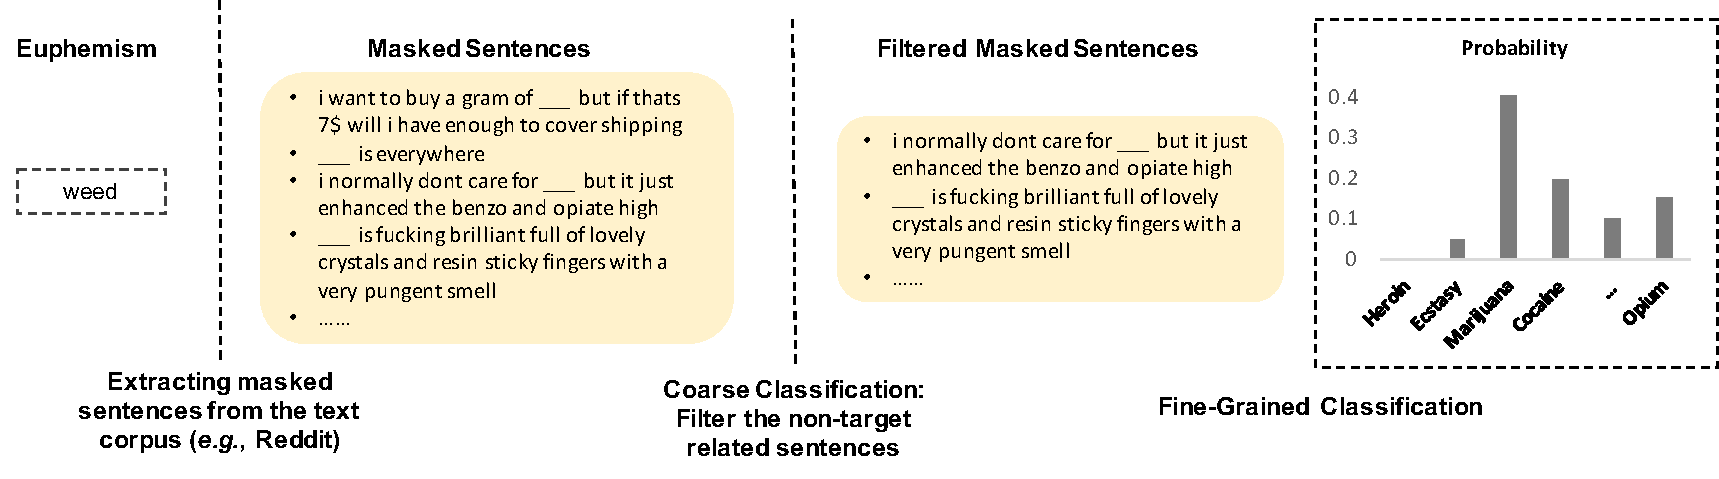
\includegraphics[width=1.00\linewidth]{figures/3}
	\caption{An overview of the euphemism identification framework.}
	\label{fig:model_iden}
\end{figure*}

Once the euphemisms are detected, we aim to identify what target keyword each euphemism refers to. 
Taking the second and third example sentences in Table \ref{table:example1}, we want to identify that ``coke'' refers to ``cocaine'' and  ``pot''  to  ``marijuana.'' 

We first discuss the challenges of the task (Section \ref{sec:iden_challenges}), and the  intuition of our approach to solve the problem (Section \ref{sec:intuition}). Finally, we present the training details of our approach (Section \ref{sec:iden_approach}). 

\subsubsection{Challenges}
\label{sec:iden_challenges}
%\noindent \textbf{Challenges}: 
Euphemism identification has been acknowledged as a highly challenging task \cite{yuan2018reading}, due to the following key challenges: 
\begin{itemize}%[leftmargin=*]
	\item \textit{Resource challenge}: 
	No curated datasets that are publicly available are adequate to exhaustively learn a growing list of mappings between euphemisms and their target keywords. Moreover, it is unclear what linguistic and ontological resources one would need to automate this task.  
	\item \textit{Linguistic challenge}: 
	The distinction in meaning between the target keywords  (\eg, cocaine and marijuana) is often subtle and difficult to learn from raw text corpora alone. 
	Even human experts are unable to accurately identify what a euphemism refers to by looking at a single  sentence. 
	On the other hand, having access to a larger number of  sentences where the euphemism occurs, provides more context to analyze the nuances between different contexts, and enables identifying what the euphemism refers to. 
	A second linguistic challenge is related to the ambiguity of the euphemism itself. 
	A given euphemism can  be used in a euphemistic or non-euphemistic sense, adding the extra layer of linguistic nuance (Table \ref{table:example4}). 
\end{itemize}


%To the best of our knowledge, no prior work has explicitly captured the meaning of a euphemism except for a few peripheral works   that identify the hypernym of a euphemism, as in ``sedative'' for a drug-related euphemism  (\eg, \cite{yuan2018reading}). 
%\nicolasc{didn't we say this in related work? paragraph candidate for deletion}
%Answer to Nicolas: removed. 

\subsubsection{Intuition}
\label{sec:intuition}
\WZ{Taking the awesome advices from Suma and Nicolas, I restructured the Intuition. How does it read now?}
We systematically address each of these challenges by a self-supervised learning scheme and a coarse-to-fine-grained classification framework. 
The key novelty lies in how we formulate the problem and solve it without additional linguistic resources or supervision. 

%To tackle the aforementioned challenges, a natural solution would be to avail a euphemism inventory---a list with each euphemism mapped to each target keyword---and then check whether the word is used euphemistically or not. % costly to collect the labels for every dataset. 
We address the \textit{resource challenge} with a self-supervised learning scheme. 
Self-supervised learning is a form of unsupervised learning where the data provides the supervision to automatically extract the training instances and their labels from an unlabeled raw text corpus. This is done by using part of a data (\eg, a sentence without a specific word), in order to predict   the remaining part of the data (\eg, the specific word of the sentence). This approach permits us to harness the abundant and readily available unlabeled data and go beyond expensive human labelling, and is especially useful for our task.  
More specifically, we extract all sentences that include the target keywords (\eg, cocaine, marijuana, heroin), mask the target keywords, and consider the masked sentences as training instances. 
This permits us to automatically construct a labeled dataset, where the instances are the masked sentences and their respective target keywords are labels. 

To address the \textit{linguistic challenge}, we adopt a coarse-to-fine-grained classification scheme, for its better discriminative performance in various tasks \cite{huo2019coarse,liu2018global,li2019exploiting}. 
The coarse classifier is a binary classifier, to examine whether the sentence is related to the specific category (\eg, drug) or not. 
It aims to filter out sentences where the euphemism words do not occur in a euphemistic sense. 
The fine-grained classifier is a multi-class classifier trained on the curated dataset from the self-supervised learning scheme, and aims to learn a specific mapping from the masked sentence to the target keyword. 



\noindent \textbf{Example}: 
Taking ``weed'' as an example, we aim to generate a probability distribution over target keywords, with most of the mass on marijuana (Figure \ref{fig:model_iden}). 
Assume that we already have a trained coarse classifier and a trained fine-grained classifer (training details will be discussed in Section \ref{sec:iden_approach}). 
We first extract all its masked sentences from the text corpus. 
Second, by the corase classifier, we filter those masked sentences that are not related to the target category (\ie, drug). 
Then, we use the filtered masked sentences as inputs to the fine-grained multi-class classifier, and obtain the target keyword label for each masked sentence. 
Now we have a list of labels for the euphemism ``weed'' (\eg, 36.1k times of marijuana, 4.2k times of ecstasy, \etc) and the final output is the label (target keyword) assigned to a majority of the euphemism's masked sentences, here \textit{marijuana}. % is a probability distribution over all the target keywords by the fraction of the number of labels. 


%To map the given euphemism to a specific target word, we construct a probability distribution over the target keywords, obtained as  the fraction of euphemism's masked sentences  labeled with a target keyword. 
%target keywords to which the masked sentences belong, is used to choose the target keyword that the euphemism maps to. 
%The target keyword with the highest probability is mapped to the euphemism.

%we adopt a supervised classification approach to learn, from their masked sentences, the nuances between different target keywords in the same category. 
%More specifically, we first train a multi-class classifier in a  self-supervised manner using the automatically labeled dataset, to learn a mapping from the masked sentence to the target keyword. 
%Then, for each euphemism, we extract its associated masked sentences, and obtain their target keyword labels using the trained classifier. 
%In the inference stage, different masked sentences for the same euphemism may be assigned different target keywords. 
%For each euphemism, we construct a probability distribution over the target keywords assigned by the classifier, where the probability of a euphemism being a target keyword is the fraction of masked sentences of that euphemism labeled with the target keyword. 
%%We consolidate the multiple labels corresponding to the masked sentences of a given euphemism by converting the hard decisions for the different instances into a soft decision over the target keywords. We do this by obtaining the   probability distribution over the target keywords, given by the fraction of times a given target keyword was chosen. 
%\nicolasc{I agree, I found this paragraph hard to understand; I didn't modify much, because I am not sure I understand well enough how the technique works.}
%\nicolasc{I got quite lost in the intuition. I wonder if it would make sense to use a running example based on one of the earlier tables to anchor the discussion.} 
%\SB{edited: how does it read now?}
%%Finally, the output will be a probability distribution by the percentage of the target keyword labels. 





\subsubsection{Training Details}
\label{sec:iden_approach}
Two classifiers need to be trained: 1) A coarse classifier to filter out the masked sentences of euphemism words not associated with their euphemistic sense
% (and hence use masked sentences related to the target keywords)
and, 2) A multi-class classifier to determine the target keyword to which the euphemism refers. 

\noindent \textbf{Coarse Classifier}: 
The coarse classifier is a binary classifier to determine whether a masked sentence is related to the target keywords or not. 
Obtaining the positive instances is easy; we collect all the masked sentences of the target keywords (\eg, we obtain the masked sentences from Table \ref{table:example3}). 
To obtain the negative instances, we adopt a negative sampling approach \cite{mikolov2013distributed}; 
we randomly choose a sentence in the text corpus and randomly mask a token. 
Since the corpus is large and diverse, we assume the randomly chosen masked sentence is not related to the target keyword. 
To create a balanced dataset, we select as many negative instances as there are positive ones. 
This set of positive and negative instances constitutes the training set, with masked sentences and their respective labels to indicate whether a masked sentence is related to the target keywords or not. 
We use 70\% of the data instances for training, 10\% for validation, and 20\% for testing. 
We select an LSTM recurrent neural network model \cite{hochreiter1997long} with an attention mechanism \cite{bahdanau2015neural} for its ability to learn where to pay attention in the input sequence. 
We obtain 98.8\% for the training accuracy and 90.1\% of the testing accuracy. 
Our experiments also included other classification models and we discuss our selection in Section \ref{sec:ablation_coarse}. 

\noindent \textbf{Multi-class Classifier}:
As presented above in Section~\ref{sec:intuition}, we use as inputs the masked sentences and as labels the target keywords. 
As an empirical selection, we adopt the multinomial logistic regression classifier \cite{hosmer2013applied} by representing each word as one-hot encoding and each sentence as the average of its composing words' encoding. 
By using the same data splitting ratio as the coarse classifier, we obtain about 55\% on training accuracy and 24\% on testing accuracy for the drug dataset (there are 33 target names in the drug dataset and therefore a random guess accuracy would be 3.3\%). 
Results by other classification models are discussed in Section \ref{sec:ablation_fine-grained}. 

